\documentclass[12pt]{article}
%\usepackage{html}
\usepackage{hyperref}
\usepackage{graphicx}
\title{CS 571\\Homework 2}
%\addtolength{\topmargin}{-2cm}
%\addtolength{\topskip}{-2cm}
%\addtolength{\oddsidemargin}{-2cm}
%\addtolength{\evensidemargin}{-2cm}
%\addtolength{\textheight}{2cm}
%\addtolength{\textwidth}{2cm}
%\addtolength{\footskip}{-1cm}
\date{}
\begin{document}
\maketitle

\begin{flushleft}
\textbf{Due}: Oct 19\hfill\textbf{100 points}\\

\textbf{No Late Submissions}

\vspace{0.5cm}

\textbf{Important Reminder}: As per the course Academic Honesty
Statement, cheating of any kind will minimally result in receiving an
F letter grade for the entire course.

\vspace{0.5cm}
To be submitted on paper in class.

\end{flushleft}

\begin{enumerate}

\item On a particular 32-bit architecture, a stack frame for a
  function with \verb@n@ parameters and \verb@m@ local variables is laid
  out as follows:

  Parameter \verb@n@ at offset \verb@4 * (n + 1)@ from the frame-pointer\\
  ...\\
  Parameter 1 at offset \verb@8@ from the frame-pointer\\
  Return address at offset \verb@4@ from the frame-pointer\\
  Saved frame-pointer at offset \verb@0@ from the frame-pointer\\
  Local variable 1 at offset \verb@-4@ from the frame-pointer\\
  Local variable 2 at offset \verb@-8@ from the frame-pointer\\
  ...\\
  Local variable \verb@m@ at offset \verb@-4*m@ from the frame-pointer.

  Assuming that the stack-frame contains only the above:

  \begin{enumerate}
  \item Give a formula in terms of \verb@n@ and \verb@m@ for the size
    (in bytes) of a stack-frame.

  \item Given the function

\begin{verbatim}
     f(int a, int b, int c) { //parameters a, b, c
       var d, e, f, g;        //local vars d, e, f, g.
        ...
     }
  \end{verbatim}
     Show the layout of the stack-frame for an invocation of f; Your
 answer should include the offset from the frame-pointer of each parameter
and local variable. \hfill{\textit{15-points}}


    \end{enumerate}

\item Given the following program in a statically-scoped language
 which supports nested functions:

\begin{verbatim}
f(a, b) {                 //1

  var x = ...;            //2

  g(a, x) {               //3
    var x = ...;          //4

    h(b) {                //5
      var a = ...;        //6
      return a + b*x;     //refs to a, b, x.
    }
  
    //body of g()
    return b + h(a)*x;    //refs to a, b, x.
  }

  //body of f()
  return a*b + x;         //refs to a, b, x.
}
\end{verbatim}

Local variable declarations are indicated using \verb@var@.  Points
$i$ where variables are defined are indicated using a comment
\verb@//@$i$.

For each line above which contains a comment \verb@refs to a, b, x@,
for each referenced variable show which declaration it refers to.
\hfill{\textit{15-points}}

\item Given the following program in a language which supports
 first-class functions as well as both lexically-scoped (indicated
 using a \verb@lex@ declaration) and dynamically-scoped variables
 (indicated using a \verb@dyn@ declaration) with \verb@lambda@ used to
 define anonymous functions.

\begin{verbatim}
//declare dynamically scoped var
dyn b = 3;

//Define function f with single parameter a
f(a) {
  lex static1 = a * 2; 
  lex static2 = b; 
  //return function which takes a single parameter x.
  return lambda (x) { return x + static1*static2 + b; }
}

//Define function f with single parameter a
sub h(a) {
  dyn b = a + 5
  return f(5)
}

//print result of calling return'd function from h(3) with 
//actual parameter 5.
print h(3)(5);

\end{verbatim}

What will be printed by the above program?  Justify your answer by showing the
values of all the variables.  \hfill{\textit{15-points}}
  
\item Consider the tree structure shown in the figure below (taken from the \href{http://zdu.binghamton.edu/cs571-16f/slides/scheme/scheme.pdf}{Scheme Slides}).

  \begin{center}
    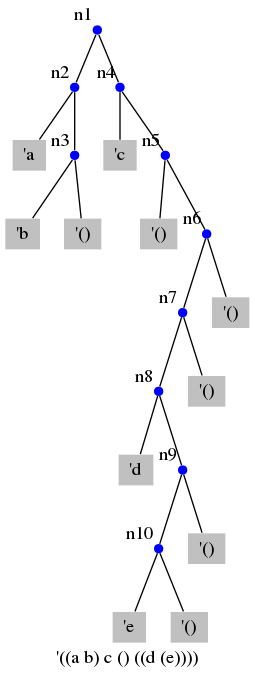
\includegraphics[height=120mm]{nest2}\\
  \end{center}

  By providing the Scheme expression equivalent to the subtree rooted
  at each internal node \verb@n1@ $\ldots$ \verb@n10@, show that the
  root node \verb@n1@ is equivalent to \verb@'((a b) c () ((d (e))))@.
  \hfill{\textit{15-points}}

\item Show that the \verb@count-non-pairs@ function discussed in the
  \href{http://zdu.binghamton.edu/cs571-16f/slides/scheme/scheme.pdf}{Scheme Slides} will always terminate. 

(Termination is usually shown by identifying some quantity which
  cannot go below some value and showing that the quantity decreases
  as the computation progresses. Since the quantity cannot decrease
  below the minimum bound, the computation must
  terminate). \hfill{\textit{10-points}}

\item How would you build conceptually infinite lists in a language
  like Scheme.  

  Specifically, if you are given

\begin{description}

\item[\texttt(next v)] 
A function which generates the next element
 in the list when given the value \verb@v@ of the previous element in
 the list.

\item[\texttt{init}] 
 A value representing the first element in the list.
\end{description}

  describe how you would build a
  data-structure which acts like an infinite list containing the
  elements generated by 0-or-more applications of the \verb@next@
  function to \verb@init@.

  For example, assume that the infinite list is constructed using the
  function \verb@(inf-cons next init)@ with parameters \verb@next@ (a
  function) and \verb@init@ (the initial value); \verb@inf-car@ and
  \verb@inf-cdr@ are accessor functions which return the head and tail
  of the constructed infinite list.  Given these definitions, it
  should be possible to build and access an infinite list of natural
  numbers as follows:

   \begin{verbatim}
     > (define inf-natnums (inf-cons (lambda (x) (+ x 1)) 0))
     > (inf-car inf-natnums)
     0
     > (inf-car (inf-cdr inf-natnums))
     1
     > (inf-car (inf-cdr (inf-cdr (inf-cdr inf-natnums))))
     3
     >   
   \end{verbatim}

   It is not required to show explicit code; it is sufficient to
   describe the essential idea.  \hfill{\textit{15-points}}
   
\item Discuss the validity of the following statements:

  \begin{enumerate}

  \item Modules form a \textit{closed scope}.

  \item The \textit{scope} of a variable is the same as it's
    \textit{lifetime}.

  \item It is possible to program without destructive assignment
    in any language which supports recursive functions.

  \item Scheme does not support destructive assignment.

    \item In Scheme, if for some expression $x$, \verb@(list?@
      $x$\verb@)@ returns \verb@#t@, then \verb@(pair?@ $x$\verb@)@
      must also return \verb@#t@. \hfill{\textit{15-points}}


  \end{enumerate}
  
\end{enumerate}


\end{document}
